\renewcommand{\mapa}{Poglavja/Slike/dvobarvna}

\begin{figure}[!ht]
    \centering
    
\includegraphics[width=0.32\linewidth]{\mapa/dvobarvna.png}
    \caption{Dvobarvna slika.}
\end{figure}

\begin{figure}[!ht]
    \begin{subfigure}{0.32\linewidth}
        
\includegraphics[width=\linewidth]{\mapa/rez35Poisson.png}
        \caption{Rekonstrukcija na 35\% znanih podatkih.}
    \end{subfigure}
    \hfill
    \begin{subfigure}{0.32\linewidth}
        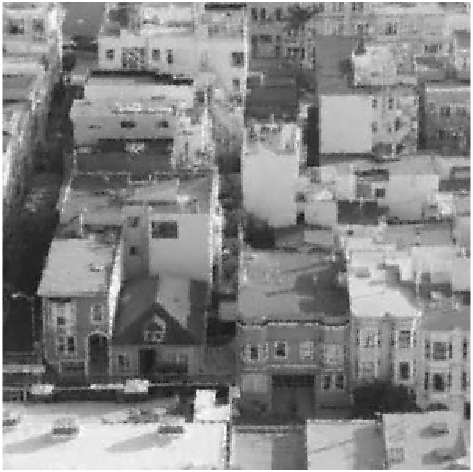
\includegraphics[width=\linewidth]{\mapa/rez45Poisson.png}
        \caption{Rekonstrukcija na 45\% znanih podatkih.}
    \end{subfigure}
    \hfill
    \begin{subfigure}{0.32\linewidth}
        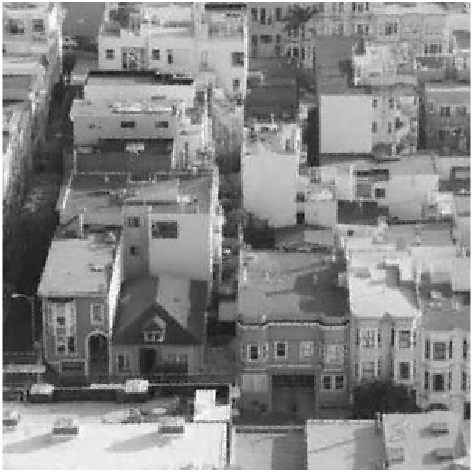
\includegraphics[width=\linewidth]{\mapa/rez60Poisson.png}
        \caption{Rekonstrukcija na 60\% znanih podatkih.}
    \end{subfigure}
\end{figure}

\begin{figure}[!ht]
    \centering
    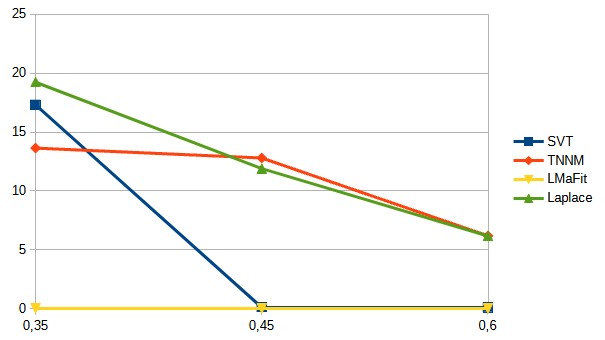
\includegraphics[width=\linewidth]{\mapa/cas.png}
    \caption{Čas izvajanja rekonstrukcije dvobarvne slike. Na abscisni osi so deleži znanih podatkov slik.}
\end{figure}